%References:
%https://www.quantstart.com/articles/Support-Vector-Machines-A-Guide-for-Beginners#ref-isl
%https://en.wikibooks.org/wiki/Support_Vector_Machines
%http://scikit-learn.org/stable/modules/svm.html
%https://cse.iitk.ac.in/users/piyush/courses/ml_autumn16/771A_lec8_slides.pdf
%http://svmlight.joachims.org/

The chosen model for the discriminative analysis is the \textit{Support Vector Machine} classifier,
an approach for classification that was developed in the computer science community in the 1990s
and has grown in popularity since then. SVM has been successfully used in many
speech processing fields, such as speaker recognition and pronunciation assessment.
% Podría incluirse alguna mención a que fue el approach discriminativo que usó el paper anterior
% The previous work of the current line proposed
% The baseline work for the current thesis developed

Given a p-dimensional feature space, an SVM (with linear kernel)
constructs a hyperplane of dimension p - 1
that separates the space in two halves, which allows to classify the instances according
to their relative position to the hyperplane \cite{svm_jwht}. The classification
procedure is then just simply a case of determining which side a test observation falls on.

If the instances are separable by a hyperplane, then there exists potentially infinite
separating hyperplanes that can be generated from those same instances, because it
is possible to slightly translate or rotate the initial plane without touching any training
observation. Among all of them, SVM generates the hyperplane that has the largest
distance to the nearest training data points of either of both classes. Such a classifier
is known as Maximal Margin Classifier, and in most of the cases generalizes better to
unobserved data than any of the other possible separating hyperplanes.

One of the key features of the Max Margin Classifier is that the location of the hyperplane
only depends on the support vectors, which are the training observations that lie directly
on the margins' boundaries.

\subsection{Soft Margin} \label{subsection:soft_margin}

One of the problems with Max Margin Classifiers is that they can be very sensitive to the
addition of new training observations: The hyperplane may be adjusted substantially
to force every instance to lie in the right side of the margin or hyerplane, thus leading
to overfitting while reducing the value of the margin (Figure \ref{fig:soft_margin_high_c}).
Moreover, many datasets are not perfectly separable via a linear hyperplane at all.
Because of these reasons, the requirement that a separating hyperplane will perfectly separate
every training observation on the correct side of the line according to its class label can
be relaxed by introducing a new concept developed in \cite{svm_soft_margin}: the Soft Margin.

\begin{figure}[H]
  \centering
  \begin{subfigure}{.5\textwidth}
    \centering
    % 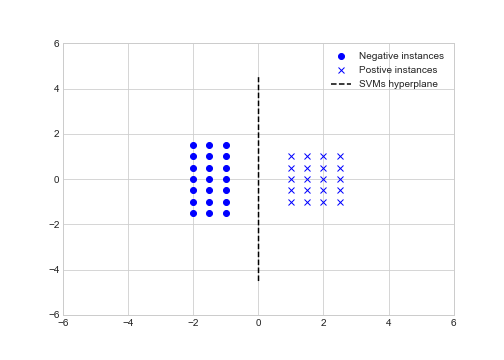
\includegraphics[width=.4\linewidth]{files/figures/method/soft_margin_normal}
    \captionsetup{width=.95\linewidth}
    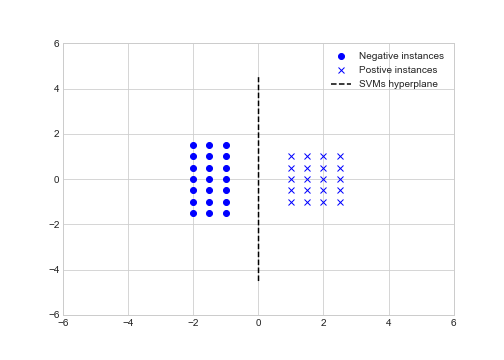
\includegraphics[width=.95\linewidth]{files/figures/method/soft_margin_normal}
    \caption{An initial training set is optimally divided by the Max Margin
    Hyperplane of an SVM}
    \label{fig:sub1}
  \end{subfigure}%
  \begin{subfigure}{.5\textwidth}
    \centering
    \captionsetup{width=.95\linewidth}
    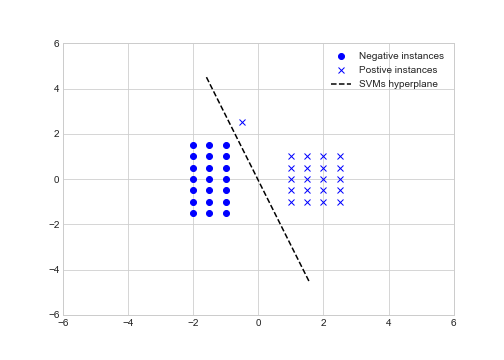
\includegraphics[width=.95\linewidth]{files/figures/method/soft_margin_high_c}
    \caption{The additon of a single instance substantially modifies
    the position of the hyperplane.}
    \label{fig:sub2}
  \end{subfigure}
  \caption{Margin adjustment when inserting a new training instance}
  \label{fig:soft_margin_high_c}
\end{figure}

A Support Vector Classifier or Soft Margin Classifier allows some observations to be on the
incorrect side of the margin or even on the incorrect side of the hyperplane, thus providing
a ``soft'' separation. The soft margin method will choose a hyperplane that splits the example
as cleanly as possible while still maximizing the distance to the nearest training instances.
The effects of the soft margin can be observed in Fig. \ref{fig:soft_margin_low_c}.

Given a labeled dataset D of $n$ tuples
of the form: $D=\{ \ (x_{i}, y_{i}) \ | \ x_{i} \in \mathbb{R}^{p}, \ y_{i} \in \{-1, 1\} \ \}$, the
problem can be formulated as:

\begin{equation}
  \displaystyle \min_{\omega, \xi} \left\{ \frac{1}{2}{\| w \|}^{2} + C \sum_{i=i}^{n}\xi_{i} \right\}, \ s.t \ \forall i: \
  y_{i}*(\omega^{t} \cdot x_{i} + b \ ) \geq 1 - \xi_{i}, \ \xi_{i} \geq 0
  \label{eq:svm}
\end{equation}

Each $x_{i}$ is a p-dimensional real number vector.
The hyperplane $\omega^{t} \cdot x + b = 0$ splits the space in two halves.
The condition $y_{i}*(\omega^{t} \cdot x_{i} + b) \geq 1$ for any instance $x_{i}$ is
known as the margin condition,
and ensures a margin $\gamma$ on each side of at least
$\frac{1}{\| \omega \|}$:

\begin{equation}
  \gamma = \frac{ |\omega^{t} \cdot x_{i} + b| }{ \| \omega \| } \geq \frac{1}{\| \omega \|}
\end{equation}

Finally, slack variables $\xi_{i}$ allow the individual observations to be
on the wrong side of the
margin or hyperplane, while $C$ is an input parameter that determines the cost of
the errors, thus establishing a trade off between a large margin and the error penalty.

\begin{figure}[H]
  \centering
  % \captionsetup{width=.95\linewidth}
  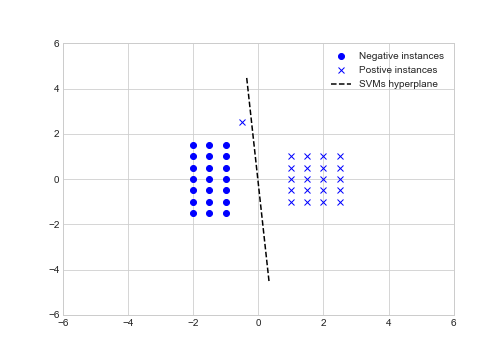
\includegraphics[width=.55\linewidth]{files/figures/method/soft_margin_low_c}
  \caption{When lowering the cost of misclassifications ($C$ parameter), the SVM still
  prioritizes maximizing the margin, though
  it allows an instance to end in the wrong side
  of the hyperplane.}
  \label{fig:soft_margin_low_c}
\end{figure}

% To conclude this section, it is worth mentioning that feature scaling is an important
% step to be performed before training
% the linear SVM classifier to avoid the dominance of the
% features with highest values
% when calculating the hyperplane. For this reason both supervectors
% and dynamic features are standardized by removing the mean and scaling to unit variance
% before training.
